\section{Evaluation}

\begin{frame}
  \frametitle{Evaluation}

  \begin{itemize}
  \item Up to 64 nodes emulated in the \acf{CORE}
  \item Nodes are connected pairwise in a chain topology
  \item Simulated IEEE 802.11g network, 54 MBit/s
  \end{itemize}

  \begin{figure}
    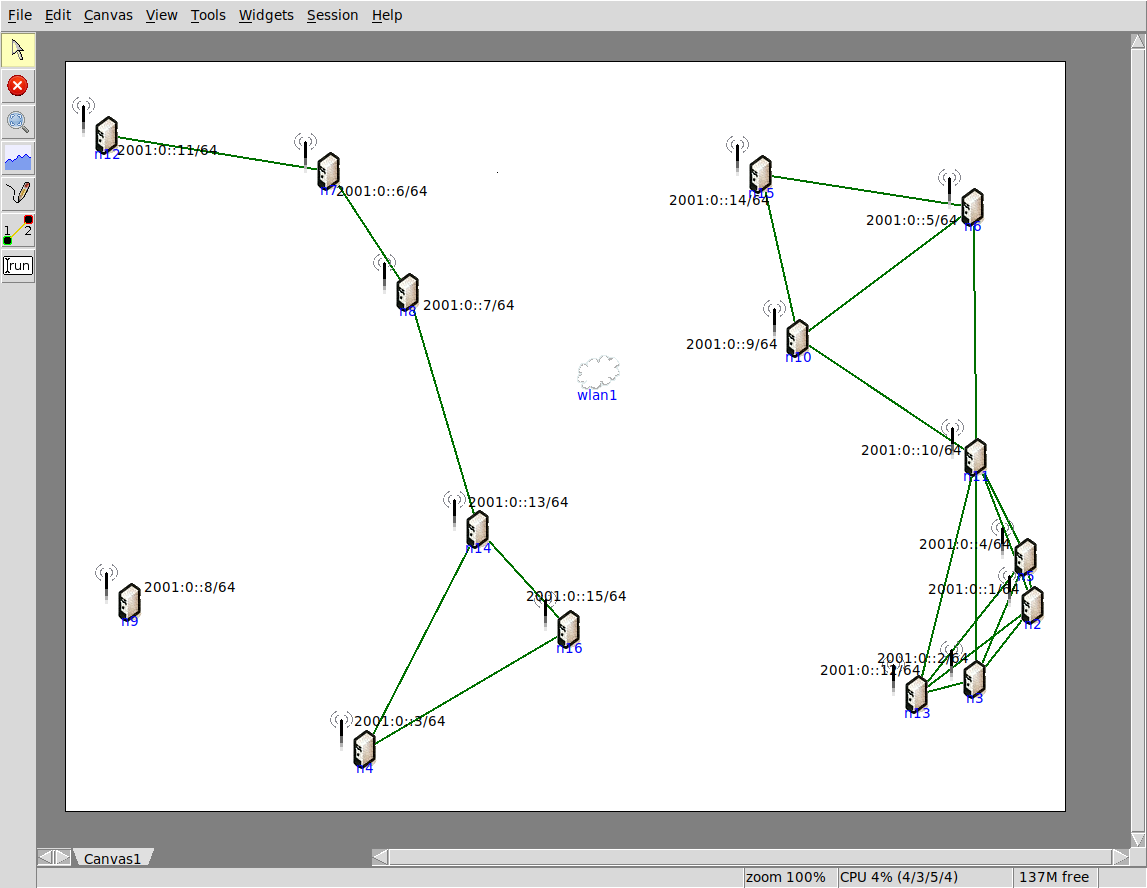
\includegraphics[width=0.8\linewidth,keepaspectratio]{include/core-screenshot}
  \end{figure}
\end{frame}

\begin{frame}
  \frametitle{Evaluation}

  \begin{itemize}
  \item Payload Size
  \begin{itemize}
    \item 64 KiB: compressed image
    \item 1 MiB: small image / short audio recording
    \item 5 MiB: smartphone image / audio recording
    \item 25 MiB: longer audio recording / short video
    \item 50 MiB: HD video
    \item 100 MiB: 4K smartphone video
  \end{itemize}
  \onslide<2>{
  \item{\acs{DTN} Software}
  \begin{itemize}
    \item DTN7
    \item Forban
    \item IBR-DTN
    \item Serval
  \end{itemize}
  }
  \end{itemize}
\end{frame}

\subsection{Results}

\begin{frame}
  \frametitle{Transmission Time: Two Nodes}

  \begin{figure}
    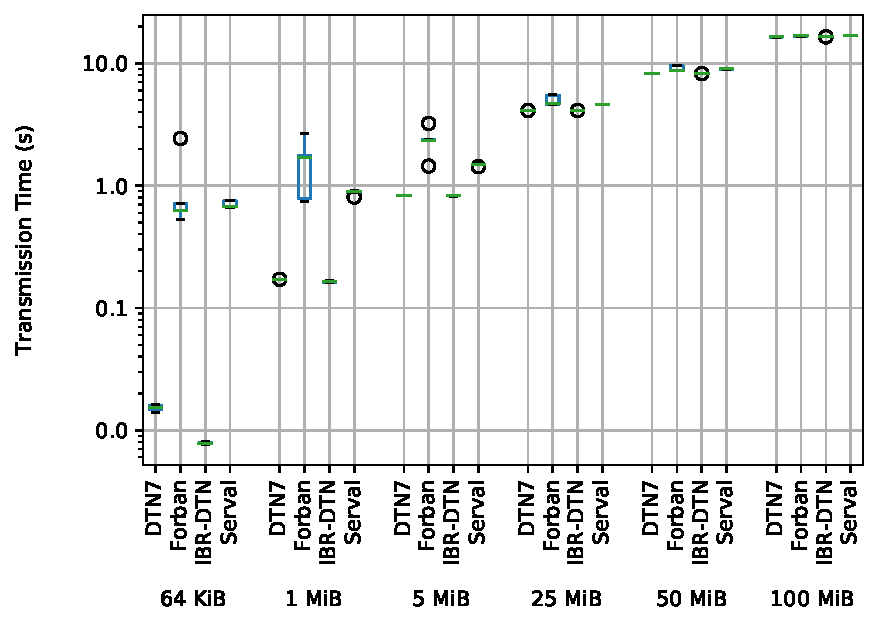
\includegraphics[width=0.8\linewidth,keepaspectratio]{include/chain-runtimes-2}
  \end{figure}
\end{frame}

\begin{frame}
  \frametitle{Transmission Time: 64 Nodes}

  \begin{figure}
    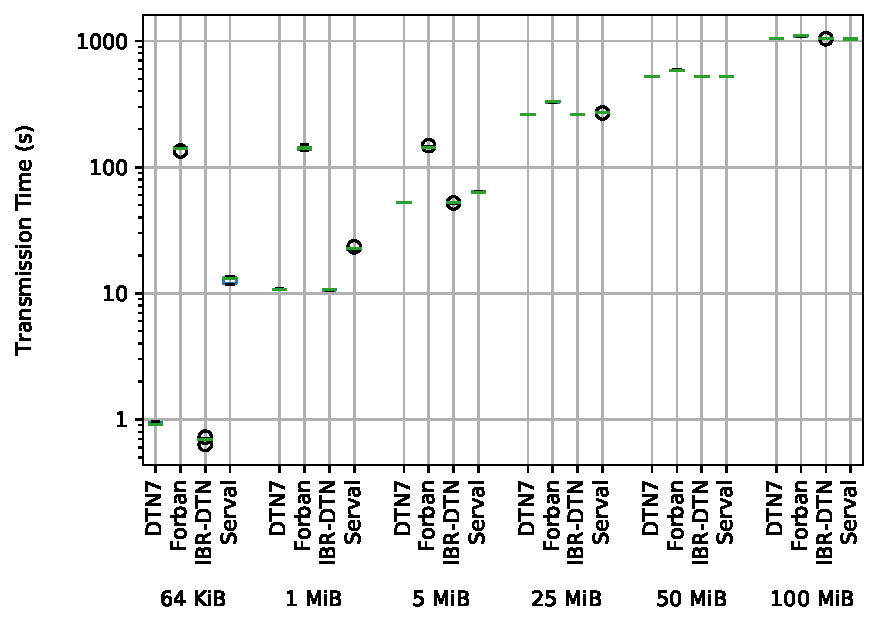
\includegraphics[width=0.8\linewidth,keepaspectratio]{include/chain-runtimes-64}
  \end{figure}
\end{frame}

\begin{frame}
  \frametitle{CPU and Network Usage: 25 MiB, 32 Nodes}

  \begin{figure}
    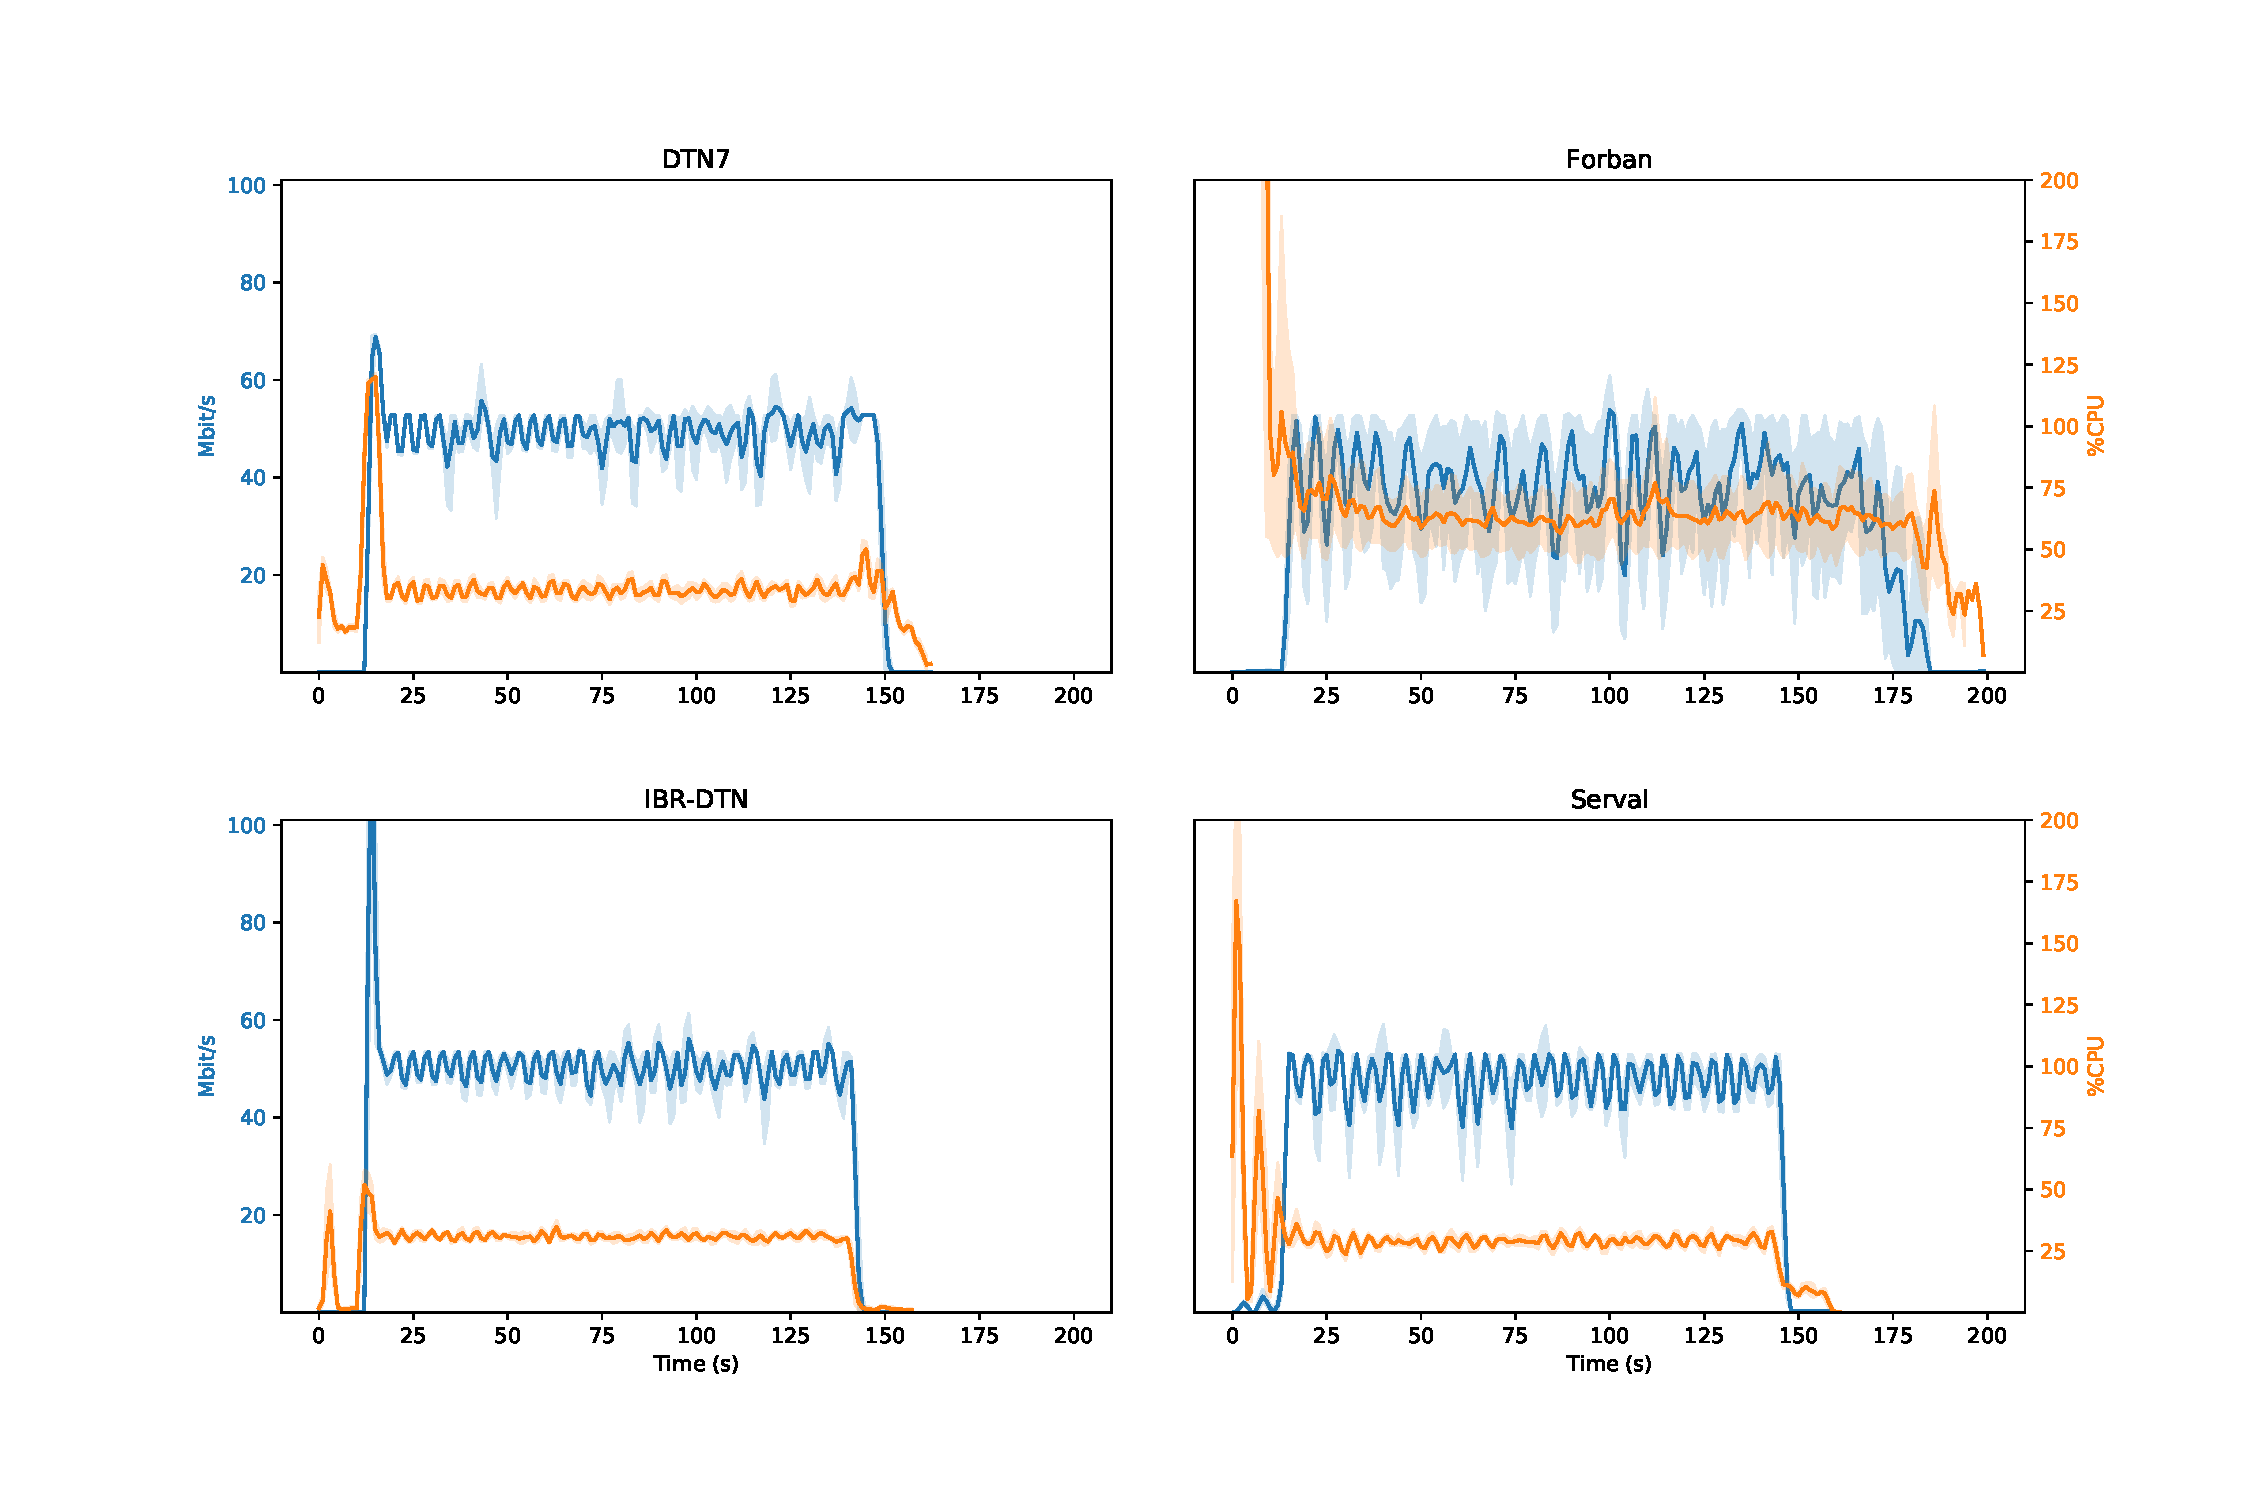
\includegraphics[width=0.9\linewidth,keepaspectratio]{include/cpu-load}
  \end{figure}
\end{frame}
